% This is samplepaper.tex, a sample chapter demonstrating the
% LLNCS macro package for Springer Computer Science proceedings;
% Version 2.20 of 2017/10/04
%
\documentclass[runningheads]{llncs}
%
\usepackage{graphicx}
% Used for displaying a sample figure. If possible, figure files should
% be included in EPS format.
%
% If you use the hyperref package, please uncomment the following line
% to display URLs in blue roman font according to Springer's eBook style:
% \renewcommand\UrlFont{\color{blue}\rmfamily}

\begin{document}
%
\title{Capstone Project Report}
%
%\titlerunning{Abbreviated paper title}
% If the paper title is too long for the running head, you can set
% an abbreviated paper title here
%
\author{Jason A. Ballard}
%
\authorrunning{J. Ballard}
% First names are abbreviated in the running head.
% If there are more than two authors, 'et al.' is used.
%
\institute{Northwest Missouri State University, Maryville MO 64468, USA \\
\email{S000000@nwmissouri.edu}}
%
\maketitle              % typeset the header of the contribution
%
\begin{abstract}
The abstract should briefly summarize the contents of the paper in
150--250 words. The abstract should briefly summarize the contents of the paper in
150--250 words. The abstract should briefly summarize the contents of the paper in
150--250 words. The abstract should briefly summarize the contents of the paper in
150--250 words.

\keywords{mobile computing \and mobile usability \and multimedia \and cloud computing}
\end{abstract}
%
%
%
\section{Introduction}

Please note that the first paragraph of a section or subsection is
not indented. The first paragraph that follows a table, figure,
equation etc. does not need an indent, either.

Subsequent paragraphs, however, are indented.

\subsection{Goals of this Research} 
Specify exactly your aims of this paper. Also, write a sentence how you will address for each individual goal.

\subsection{This is another subsection}
Write something related to your paper.

\section{Mobile Usability}


\begin{table}
\caption{Gas Prices}\label{gasprice}
\begin{tabular}{|l|r|}
\hline
Month &  Price \\
\hline
Jan &  \$2.12 \\
Feb &  0.12 \\
Mar &  1.12 \\
Apr &  2.12 \\
May &  3.12 \\
Jun &  1.12 \\

\hline
\end{tabular}
\end{table}



\begin{table}
\caption{Table captions should be placed above the
tables.}\label{tab1}
\begin{tabular}{|l|l|l|}
\hline
Heading level &  Example & Font size and style\\
\hline
Title (centered) &  {\Large\bfseries Lecture Notes} & 14 point, bold\\
1st-level heading &  {\large\bfseries 1 Introduction} & 12 point, bold\\
2nd-level heading & {\bfseries 2.1 Printing Area} & 10 point, bold\\
3rd-level heading & {\bfseries Run-in Heading in Bold.} Text follows & 10 point, bold\\
4th-level heading & {\itshape Lowest Level Heading.} Text follows & 10 point, italic\\
\hline
\end{tabular}
\end{table}


The gasoline prices are summarized in Table \ref{gasprice}



\noindent Displayed equations are centered and set on a separate
line.
\begin{equation}
x + y = z
\end{equation}
Please try to avoid rasterized images for line-art diagrams and
schemas. Whenever possible, use vector graphics instead (see
Fig.~\ref{fig1}).

\begin{figure}
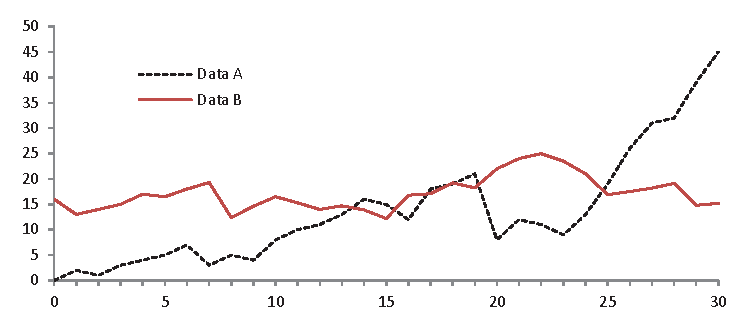
\includegraphics[width=\textwidth]{fig1.eps}
\caption{A figure caption is always placed below the illustration.
Please note that short captions are centered, while long ones are
justified by the macro package automatically.} 
\label{fig1}
\end{figure}

The detailed steps of the MEC is shown in Figure \ref{mecFig}.

\begin{figure}
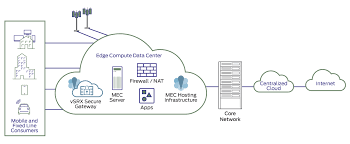
\includegraphics[width=\textwidth]{mecomputing.png}
\caption{This is the MEC} 
\label{mecFig}
\end{figure}

%\begin{theorem}
%This is a sample theorem. The run-in heading is set in bold, while
%the following text appears in italics. Definitions, lemmas,
%propositions, and corollaries are styled the same way.
%\end{theorem}
%
% the environments 'definition', 'lemma', 'proposition', 'corollary',
% 'remark', and 'example' are defined in the LLNCS documentclass as well.
%
\begin{proof}
Proofs, examples, and remarks have the initial word in italics,
while the following text appears in normal font.
\end{proof}


The following are the items in my lunch menu.
\begin{itemize}
    \item Fish
    \begin{itemize}
        \item sauce
        \item fires
    \end{itemize}
    \item Chicken
    \item Yogurt
    \item ice cream
\end{itemize}

The following are the steps to cook this recipe. 



\begin{enumerate}
\item Clean vessels
\item Cook
\begin{enumerate}
    \item On the stove
    \item Place the pan
    \item Crack the egg
\end{enumerate}
\item Eat
\end{enumerate}



For citations of references, we prefer the use of square brackets
and consecutive numbers. \cite{bariah2020prospective}, \cite{kato2020ten}.

Now I am citing this article. \cite{hoehle2015mobile}

citing now \cite{8766917}, \cite{10.5555/2667432.2667458}

Now, I am using my sixth \cite{mao2017survey} citation.

\cite{910896}

\cite{*}

%
% ---- Bibliography ----
%
% BibTeX users should specify bibliography style 'splncs04'.
% References will then be sorted and formatted in the correct style.
%
\bibliographystyle{splncs04}
\bibliography{mybibliography}


%

\end{document}

